\chapter{Background}
\label{chap:background}
\lhead{\emph{Background}}
\section{Thematic Area within Computer Science}
This project is focused on developing a docker linter for best practices by combining multiple areas within the computer science field. 
The aim of the paper is to propose a Docker linter that enforces best practices, improving the quality of Dockerfile through the detection of Docker smells and automated refactoring suggestions. This paper has proposed a Docker Linter, which checks Dockerfiles to see whether best practices defined by the industry and best configuration practices are applied and gives recommendations to developers that can actually be acted upon. This tool will assist developers and DevOps engineers in building secure, efficient, and maintainable Docker images by automatically detecting configuration issues, ensuring consistency, and reducing human errors. Unlike other tools focused purely on vulnerability detection, this project focuses on Dockerfile optimisation and best security configuration practices at the code level.
% notice the enumerate structure to create itemized lists
\subsection{Core Topic of Project.}
    This core idea is to develop a Docker linter that parses Dockerfiles for adherence to best practices and detection of "Docker smells", which means violations of best practices and may affect Docker image security, performance, and maintainability. With the focus on optimisations at the Dockerfile level, this linter satisfies that need for a tool to improve Dockerfile quality without the use of other external services for vulnerability detection.\cite{StudyofDockerSmells}
    
\subsection{Software Engineering}
    Software Engineering is a key area in this project, focusing on maintaining and refactoring Dockerfiles without changing the external outcome.
    Software Engineering has the objective to solve industry's problems by producing good, maintainable software.\cite{softwareEng}
    The linter uses static code analysis, a software engineering technique that examines code without executing the program. This provides an understanding of the code structure and can help ensure the code adheres to the best practices. 
    
    This project aligns with software maintenance approaches since it provides continuous updates to Dockerfile best practices, ensuring that teams are always equipped with the latest rules and recommendations.Software maintenance, refers to the continuous improvement of the software artifacts\cite{canfora2001softwaremaintenance}. Docker Linter, in the context of this present project, would go a long way toward keeping teams current with the evolving best practices in Dockerfiles and hence reduces the risk of \textit{Docker Smells}, which are violations of best practices, similar to code smells \cite{DockerSmellEmpherical}. This project's automation of quality assurance ensures consistent code reviews that are less susceptible to human errors, thus adhering to principles of software engineering such as automation, consistency, and repeatability. \cite{softwareEng}
    
    It also generalises the notion of refactoring, known in software engineering as improving code or configuration files to a higher quality without changing their external behaviour. \cite{refactoring} In this case, refactoring means rewriting Dockerfiles for compliance with the best practices and avoiding Docker anti-patterns. This would allow a developer to enforce a single coding standard, thereby improving the overall collaboration within the development group and the quality of the code.
\subsection{Virtualisation}
    Virtualization is the process of creating virtual instance of a computer system.\cite{ConVSVirt} Virtualisation enhances resource efficiency and utilisation by enabling the independent operation of numerous operating systems and applications on a single physical computer by abstracting the underlying hardware. Virtual Machines (VMs) are primary products of virtualisation. A VM includes its own operating system, libraries and application files, enabling isolation between applications and underlying host systems. Each VM runs on a hypervisor which is virtual machine monitor, which means they run and monitor VMs\cite{ConVSVirt}
   
    Virtualisation has been a part of the computing scene for nearly half a century.In the 1960s and 1970s IBM developed the Control Program which led into VM/370.\cite{Virt2013} These Systems let each user run what seemed to be an isolated system, but all within a timeshared computing environment.Virtualisation has advanced dramatically over the years and is now a fundamental component in modern computing environments. The desire to maximise resource utilisation, increase system scalability, and improve isolation for security and stability have driven the development of virtualisation technologies. These earlier ideas have been expanded into enterprise-grade solutions by contemporary hypervisors like VMware ESXi, Microsoft Hyper-V, and open-source programs like KVM and Xen.\cite{Virt2013}

    The ability of virtualisation to enhance resource utilisation is one of its main contributions to this project. Multiple VMs can share physical hardware in virtualised settings, which improves resource use efficiency. By eliminating unnecessary image layers, requiring multi-stage builds, and eliminating unneeded dependencies, the Docker Linter also seeks to encourage resource-efficient Dockerfiles. This is similar to virtualization's objective of guaranteeing lean and optimised infrastructure, which is especially advantageous in cloud-native settings where resource efficiency and performance are crucial.\cite{2012virtualization}

    Despite its benefits, virtualization has limitations that highlight the value of containerization. The resource overhead of VMs, which require a full operating system, is significantly higher compared to lightweight containers that use OS-level virtualization. This project leverages the lightweight nature of containers by promoting best practices through the Docker Linter, ensuring that containerized applications remain efficient, agile, and scalable without the bulkiness of traditional VMs.\begin{figure}[ht]
  \centering
  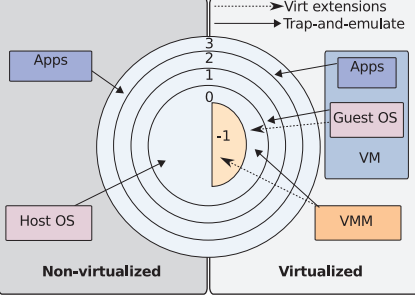
\includegraphics[width=0.63\textwidth]{Figures/Virt.png}
  \caption{overview of non-virtualized and virtualized application environments, \cite{2012virtualization}} % Use braces {} for the caption text
  \label{fig:2.2} % Ensure unique label
\end{figure}

In \ref{fig:2.2} provides a comparative overview of non-virtualised and virtualised application environments, emphasizing the abstraction and layering involved in virtualization. On the left, the non-virtualised setup demonstrates a direct relationship between applications and the host operating system, which manages the hardware resources directly. This approach is simpler but lacks isolation, making it less secure and efficient for running multiple applications concurrently.

On the right, the virtualised environment introduces additional layers of abstraction. Applications run within their own isolated virtual machines (VMs), each containing a guest operating system (OS). The hypervisor or Virtual Machine Monitor (VMM) lies beneath the VMs, providing resource allocation and ensuring the separation of environments. The hardware-level virtualisation is managed through mechanisms like trap-and-emulate or virtualization extensions, which enable the hypervisor to efficiently simulate the hardware for each VM.

This diagram highlights the key benefits of virtualisation, such as enhanced resource sharing, isolation, and flexibility, as each VM operates independently. However, it also underscores the added complexity and overhead introduced by managing virtual machines, making a compelling case for lightweight alternatives like containerisation in certain scenarios.

\subsection{Containerisation}
This project relates closely to Containerisation as Docker provides a way to deploy, maintain and run applications in the cloud. Containers have gained popularity as a lightweight alternative to virtual machines, particularly in micro services, due to their resource efficiency, scalability and flexibility. Containerisation has seen rapid growth in recent years but the one main barrier to adoption is security.\cite{sultan2019container}  In cloud environments, apps are deployed in containers, this allows for scalability as Kubernetes can automatically scale the container up or down depending on demands, better utilisation as containers use OS-level virtualisation rather than creating a separate VM, and flexibility as containers can be assigned specific CPU and memory. \cite{hardikar2021containerization}

This is important when one is performing application deployments at scale across cloud environments, and for this, the linter ensures that Docker images are optimised for performance.The linter does this by reducing unnecessary layers, enforcing multi-stage builds, and getting rid of unused dependencies, among other things, to make the Docker images minimal in size.\cite{DockerSmellEmpherical}

The Docker Linter also contributes to scalability by optimising images for horizontal scaling,where containers may be dynamically increased or decreased based on application load. The linter will aid the developer to achieve Lean, streamline images which will reduce deployment time, leading to faster response during high-load situations, it will also help decrease the attack surface, addressing docker smells and help reduce the barrier to adoption. \cite{StudyofDockerSmells}

The linter also supports operational efficiency, automating optimisation to help continuos deployment.This aligns with the goals of cloud native development, where agility, scalability and security are essential. 

This project generally aims at promoting Docker for cloud native development by offering a comprehensive way to enhance the quality of the container image, reduce cloud infrastructure costs, and ensure reliable deployments. Docker linter helps an organisation deploy more efficient, secure, and agile containers that will help to achieve a robust yet cost-effective cloud-native strategy. 

In \ref{fig:2.3} We can see the relationship between the applications, docker, the host operating system and the underlying infrastructure. At the top we can see multiple application running independently within containers which allows for isolation and efficient resource usage. 
The Docker layer sits below the applications, functioning as container runtimes that manage each container's execution environment. This setup relies on OS-level virtualisation, where containers share the same host OS kernel but remain isolated from one another, allowing resource efficiency without the need fir separate virtual machines. 
Beneath the Docker layer, The host operating systems manages the hardware by interacting with the underlying infrastructure.
This layered architecture shows the key benefits of containerisation; each application is isolated but runs on shared infrastructure, supporting scalability, flexibility and resource efficiency. 
\begin{figure}[ht]
  \centering
  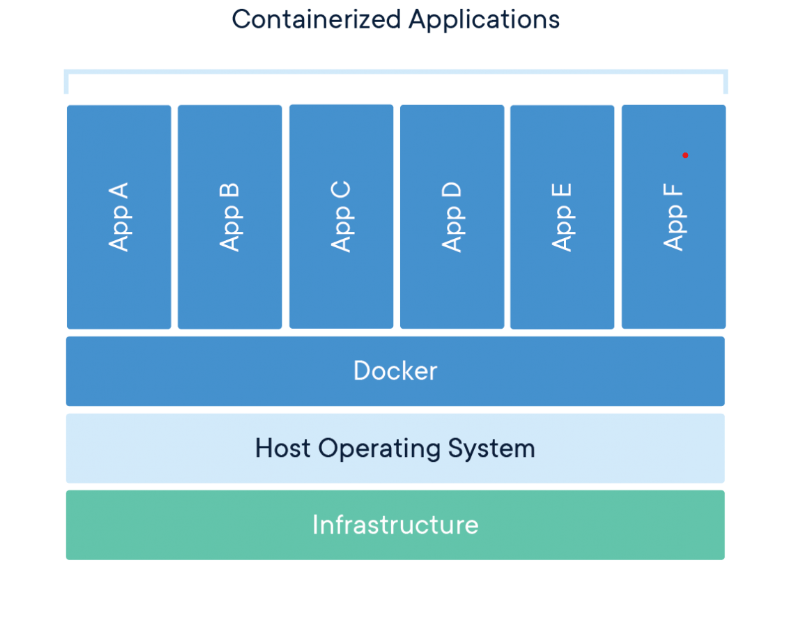
\includegraphics[width=0.73\textwidth]{Figures/container_diagram.png}
  \caption{Overview of a containerised application environment \cite{docker_cont}} % Use braces {} for the caption text
  \label{fig:2.3} % Ensure unique label
\end{figure}

\subsection{Containerisation Vs Virtualisation}
Containerisation and virtualisation are two fundamental technologies in modern computing that enable efficient utilisation of resources and application isolation, both come with several advantages and disadvantages mostly over each other.As these are both used for a wide range of application and can be used for different purposes, choosing one over the other can be of significant importance.\cite{ConVSVirt}

Virtualisation provides robust isolation and compatibility for diverse operating systems, making it a key technology in scenarios where strong security and support for legacy applications are critical.By creating fully isolated VMs, each with its own operating system, libraries and applications, virtualisation ensures that the failure of one VM does not affect others.This is important for multi-tenant environments, where security concerns are essential due to shares hardware among different users or clients.\cite{Virt2013}
However,this robust isolations comes at a cost, it introduces overhead, each VM requires substantial resources because of the need to replicate operating systems. The hypervisor, which manages these VMs add further overhead, resulting in reduced memory efficiency when compared to containerisation. 

In contrast, containerisation offers lightweight alternative that abstracts the operating system rather than the hardware. Containers share the the host OS kernel,which eliminates the need for multiple operating system instances, reducing the resource consumption.\cite{2022containerization}
This shared-kernel approach allows containers to be more agile, starting in seconds and consuming far fewer resources than VMs.\cite{Con2014docker}
However, containerisation does have limitations. While it is highly efficient, the shared-kernel model means that containers are less isolated than VMs. If the host OS is compromised, all containers running on that host are potentially at risk. In contrast, virtualisation provides stronger boundaries between applications, as each VM operates independently, with its own OS and security context. As a result, virtualisation is still highly relevant in scenarios where stronger isolation is required, such as in handling sensitive workloads or running software with strict compliance requirements.

The trade-offs between virtualization and containerization provide important context for this project. Understanding virtualization highlights the challenges that containerization overcomes, such as resource overhead and slower startup times. However, it also emphasizes the need for careful security practices in containerized environments, as containers do not provide the same level of isolation as VMs. The Docker Linter plays a crucial role in mitigating these risks by promoting best practices that reduce the attack surface, such as minimizing the number of layers, avoiding unnecessary dependencies, and enforcing the use of non-root users in containers.

\begin{figure}[ht]
  \centering
   \rotatebox{-90}{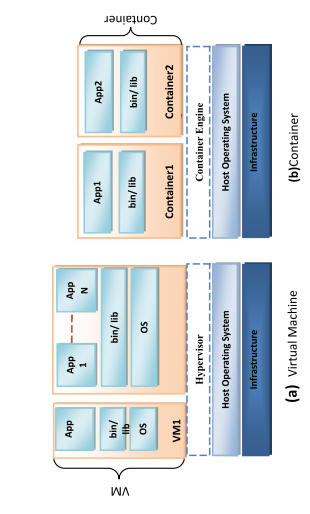
\includegraphics[width=0.63\textwidth]{Figures/Cont 143619.png}}
  \caption{fundamental differences between virtualization and containerization \cite{2022containerization}} % Use braces {} for the caption text
  \label{fig:2.4} % Ensure unique label
\end{figure}

\ref{fig:2.4} highlights the fundamental differences between virtualization and containerization, focusing on their architecture and resource utilization. Virtualization relies on hypervisors to create virtual machines (VMs), with each VM containing its own operating system, libraries, and applications. This model ensures strong isolation and compatibility for diverse workloads but comes with significant resource overhead due to the duplication of operating systems.

In contrast, containerization leverages a container engine, such as Docker, to run multiple lightweight containers that share the host operating system. Containers are more resource-efficient, as they avoid duplicating the OS, and they start quickly, making them ideal for modern cloud-native applications. The shared OS kernel and absence of hypervisor overhead allow containers to scale dynamically and deploy faster.

This distinction is crucial for the Docker Linter project, as it focuses on optimizing containerized workflows. By reducing unnecessary layers and enforcing best practices, the linter ensures containers remain efficient, scalable, and agile, aligning perfectly with the benefits of containerization depicted in the diagram.

\subsection{Docker Architecture and operational layers}
Docker's layered architecture simplifies the complicated process of application deployment and management.The figure \ref{docker_lies} shows how the programs are seperated, managed and run on the underlying hardware.

\subsubsection{Physical Sever}
At the bottom of the stack is the physical hardware, which provides the foundation for all higher layers.This includes the CPU, memory and storage necessary to run the operating system. 
\subsubsection{Operating System}
This manages the hardware and provides essential services. Docker relies on the host OS for key functionalities, such as kernel-level operations, process scheduling,etc. 
\subsubsection{Docker Engine}
The docker engine is the main layer that enables containerisation (as discussed above). The Docker Engine consists of three main components: 
\begin{itemize}
    \item \textbf{Docker Daemon:}creates, runs and manages container.
    \item \textbf{Docker CLI:}Provides the command line interface for user to interact with Docker.
    \item \textbf{Container Engine:}makes it easier to create and manage containers.\cite{schenker2020learn}
\end{itemize}
The Docker Engine allows containers to share the host OS kernel while maintaining process isolation, which reduces overhead compared to virtual machines.
\subsubsection{Comparison to Virtual Machines}
The diagram also highlights how Docker differs from traditional virtualization. Virtual machines, shown on the right, require a hypervisor to manage multiple virtualized operating systems on the same physical hardware. Each VM includes its own OS, which leads to significant overhead. In contrast, Docker containers share the host OS kernel, eliminating the need for individual OS instances and providing better performance and scalability.\cite{d}


\begin{figure}[ht]
  \centering
    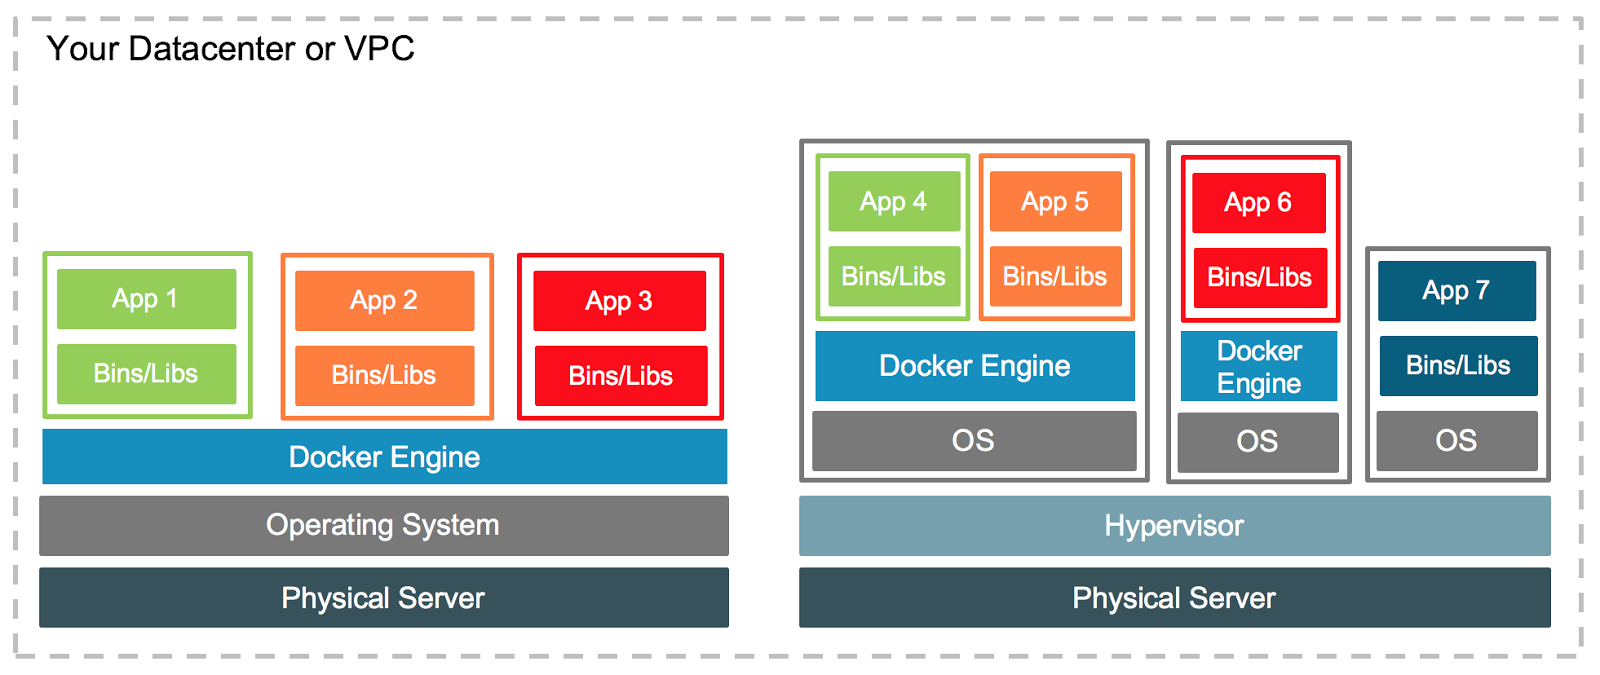
\includegraphics[width=0.93\textwidth]{Figures/difference-vm-containers.png}
  \caption{Where Docker lies \cite{docker_conttainer_where}} % Use braces {} for the caption text
  \label{docker_lies} % Ensure unique label
\end{figure}
\subsection{Docker Artifacts And Their Role}
Docker artifacts are the fundamental components generated and used throughout the Docker lifecycle.These include Dockerfiles, images, and registries, each playing a crucial role in the containerisation ecosystem. 
\begin{enumerate}
    \item \textbf{Dockerfiles:}These are the blueprint for creating Docker images. They contain the necessary instructions, such as installing the base image and copying files. A well structured Dockerfile is essential for producing an efficient, secure and scalable image.
    \item \textbf{Docker Images:}These are read only templates built from Dockerfiles.They include all the components required to run an application, such as libraries, binaries and dependencies.Images are portable and can be reused across various stages from development to production. 
    \item \textbf{Docker Registry:}A Docker registry, such as Docker Hub or private repositories, is a centralized location to store,distribute, and manage Docker images.It allows teams to share and retrieve prebuilt images for rapid deployment. \cite{DockerArtifacts}
\end{enumerate}
\subsection{Security}
 Security in this project is focused on secure configuration and best practices inside the Dockerfile itself. The linter is an application of configuration security rather than external scanning for vulnerabilities based on the detection of such risky practices as using root privilege, not specifying minimal base images, or missing secure environment configuration.
    
\textit{Shift-left} approach is the integration of continuous automated testing throughout development.
\cite{shift-left}.This will fit the concept since the security checks have been performed way in advance of the deployment. And teams can create Docker images securely. Automation of security recommendations and potential misconfiguration by Docker linter will avoid vulnerabilities with respect to Dockerfile setup. More focusing on the security through best practices rather than third-party vulnerability databases.


% Again take note of the structure, simply copy and paste this for future single figures


\section{A Review of Dockerfile quality issues and Smells}
In this section, relevant papers will be discussed in detail and how they relate to this project. Then in section 2 , similar applications will be discussed and how this project differs to them.
\subsection{Background on Docker and Its importance}
Docker is an open source tool that packages code and dependencies into a container image. It also provides an online repository for Docker images called Docker Hub.\cite{hardikar2021containerization}Unlike traditional virtual machines, which includes the OS kernel as well as the OS applications. Docker containers which are running instances of Docker Images, shares the OS kernel with the host and has it's own OS applications making it lightweight, faster and more efficient.This makes Docker a core tool in DevOps, cloud computing and containerised environments. \cite{2017Docker}

In cloud computing, Docker enables applications to be packaged and deployed,regardless of the underlying environments.Docker Desktop adds a hypervisor layer allowing the Linux applications to run on a windows or Mac OS kernel.This portability ensures that applications behave consistently across development,testing, and production stages.
In DevOps, Docker allows for continuous integration/Deployment, enabling rapid application updates, streamlined testing and seamless deployment. Containers also reduce the "it works on my machine" problem every developer faces. 

Docker's flexibility can also lead to security risks. Dockerfiles;scripts that define the instructions for building a Docker image\cite{hardikar2021containerization},play a crucial role in managing container quality and security. However without abidance to best practices, Dockerfiles can lead to containers that are bloated and hard to maintain.This veer from the best practices are called "Docker Smells". This can comprise the Docker Image security, efficiency. As companies scale their applications and rely on containers, maintaining Dockerfiles is essential to prevent vulnerabilities and security risks. Therefore, ensuring Dockerfiles adhere to best practices is essential to achieving scalable, secure and efficient images. 

\subsection{What are Dockerfile Smells?}
The concept of "Smells" comes from  software engineering where "Code Smells" are patterns in the code that indicate underlying issues or poor practices, even if they do not cause problems straight away."Docker smells" are signs of inefficient practices or configurations within Dockerfiles. These can impact a container's performance,security, or maintainability and can often lead to long-term vulnerabilities and reliability problems. 

The paper "Assessing and Improving the Quality of Docker Artifacts" \cite{DockerArtifacts} categorises these Docker smells into various types, each with it's own implications for container quality.Here are some examples of common "docker smells" and how to fix them \cite{DockerSmellEmpherical}:
\begin{enumerate}
    \item \textbf{Use of 'cd' to switch to a directory}:
    \\The WORKDIR instruction is more efficient as it sets the working directory for all subsequent instructions.It also works across build layers, making the Dockerfile more maintainable. 
    \\\textbf{FIX:} Replace \verb|RUN cd /path/to/dir| with \verb|WORKDIR /path/to/dir|. 

    \item \textbf{Missing version pinning for base image:}
    \\Having an image with the latest tag means the image will keep changing if a new version of that image is released. 
    Use specified versions. E.g Alpine. 
    \\\textbf{FIX:} Replace \verb|FROM ubuntu| with \verb|FROM ubuntu:20.04|

    \item \textbf{Missing version pinning for 'apt-get' Packages:}
    \\To ensure consistency in builds and prevent issues caused by unexpected updates in packages, pinning the version of the package ensures that image will have a stable package throughout and that any updates wont break the image or cause any security risks 
    \\\textbf{FIX:} Run \verb|apt-get install package=1.2.3| instead of \verb|Run apt-get install package|
    
    \item \textbf{Delete the apt-get lists after installing packages:}
    \\Temporary files used during package installation can bloat the image if not removed.Clearing the apt-get cache and package list after installation can reduce the image size. 
    \\\textbf{FIX:} Add \verb|RUN rm /var/lib/apt/lists/*| after \verb|apt-get install| commands.
    
    \item \textbf{Avoid Additional Packages by using '--no-install-recommends'}
    \\Using the the --no-install-recommends flag with apt-get install to prevent unnecessary packages from being installed. This Reduces the image size and minimises the potential attack surface
    \\\textbf{FIX:} Use \verb|RUN apt-get install --no-install-recommends| package. 
    
    \item \textbf{Use 'copy' instead of 'ADD' for files and Folders}
    \\Add has additional functionality (e.g extracting tar archives) that is not always needed, which can lead to unexpected behaviour.
    \\\textbf{FIX:}  Replace \verb|ADD file/path|  with \verb|COPY file/path|
    
    \item \textbf{'MAINTAINER' is deprecated:}
   \\By replacing 'MAINTAINER' with with 'LABEL', provides more flexibility and aligns with modern Docker practices.
    \\\textbf{FIX:} Replace \verb|MAINTAINER name| with \verb|LABEL maintainer='name'|
    
    \item \textbf{Set -o pipefail to avoid silencing errors in RUN instructions:}
    \\By adding \verb|SHELL ["/bin/bash","-o", "pipefail", "-c"]| to ensure errors in piped commands are not silenced.This helps in identifying errors in complex \verb|RUN|commands that use pipes.
    \\\textbf{FIX:} Add \verb|SHELL ["/bin/bash", "-o", "pipefail", "-c"]| before \verb|RUN| commands that include pipes.
    
    \item \textbf{Consolidate Multiple Consecutive RUN Instructions:}
    \\ Combining multiple \verb|RUN| instructions into a single instruction, reduces the number of layers in the Docker Image, improving build performance and reducing size.
    \\\textbf{FIX:} Replace multiple \verb|RUN| commands with one e.g 
    \begin{lstlisting}
    RUN apt-get update && \
        apt-get install -y curl wget && \
        apt-get clean && \
        rm -rf /var/lib/apt/lists/*
    \end{lstlisting}
    
    \item \textbf{Use JSON Notation for CMD and ENTRYPOINT:}
    \\Using JSON array syntax for \verb|CMD| and \verb|ENTRYPOINT|, prevents issues with shell interpretation of commands arguments, ensuring reliability. 
    \\\textbf{FIX:} Replace \verb|CMD /app/start.sh| with \verb|CMD ["app/start.sh"]|.
    
\end{enumerate}

\subsection{A literature Review of Assessing and Improving the Quality of Docker Artifacts
}
In recent years, Docker has revolutionised the way applications are developed, packaged, and deployed, becoming the backbone of cloud-native and Devops practices. Docker enables developers to create a lightweight, portable containers that encapsulates an application along with its dependencies. portability makes it easier to deploy consistently from development to diverse environments, from development to production. However, the quality of Docker artifacts, especially Dockerfiles play a crucial role in determining the overall efficiency, security and maintainability of containerised applications.

A Dockerfile serves as the blueprint for building Docker images. It's configuration determines not only the functionality of the resulting container but also, its size,build time and security.Despite its simplicity, writing optimal Dockerfiles remains a challenging task.Developers often introduce configuration flaws, known as 'Docker Smells',that compromise the effectiveness of containerisation process.These "smells" can include inefficient image layering, the use of outdated base images, and the lack of version pinning for dependencies.\cite{acharya2021docker}

The concept of "Docker Smells" draws parallels to code "smells" in traditional software development, where certain patterns indicate deeper quality issues.As identified by Giovanni Rosa, Docker smells include non-optimal practices that lead to:
\begin{enumerate}
    \item \textbf{Performance Degradation:} larger image sizes increase storage and network transfer costs, slowing down deployment pipelines.
    \item \textbf{Security Risk:} Weak configuration, such as running containers as root expose applications to potential exploits
    \item \textbf{Maintainability Challenges:} Poorly structured Dockerfiles complicate updates, leading to technical debt and slower iteration cycles. \cite{DockerArtifacts}
\end{enumerate}

The study conducted by Rosa et al, aims to assess the prevalence and impact of these "smells" across a large dataset of Dockerfiles, providing empirical evidence of their significance in real world situations.The findings reveal that these smells are prevalent and often remain unaddressed due to lack of awareness. 

"Docker smells", as explored by Rosa et al. \cite{DockerArtifacts}, are patterns of poor practices in Dockerfiles that compromise containerised application's efficiency, security and maintainability.In modern cloud native environments, the impact of these "smells" are amplified due to the scale and changeability of containers. 

\textbf{Performance Degradation} is one of the most evident consequences of Dockerfile "smells". The authors highlight that common practices, such as creating multiple layers through unoptimised \verb|RUN| commands, significantly inflate Docker image sizes. For example, each \verb|RUN| command creates a new layer in the final image, and when commands like \verb|apt-get install| are not involved in cleanup (\verb|apt-get clean|), unnecessary files are present, bloating the image. Bloated images lead to slower download times during deployment and increased storage costs, which are particularly critical in resource-constrained environments like Internet of things. \cite{securityDocker}

In terms of \textbf{security},"Dockerfile smells" introduce vulnerabilities that attackers can exploit. Running containers as root, failing to pin versions of base images, exposing unnecessary ports are practices that broaden the attack surface. Rosa et al, point out that unpinned version are particularly dangerous because they allow unintended updates to newer, potentially vulnerable versions of software components. These configurations make it harder for developers to track changes in their dependency tree, increasing the risk of deploying vulnerable containers into production environments.\cite{DockerArtifacts}

\textbf{Maintainability Issues} further worsen the challenges posed by "Docker smells". Instructions like \verb|MANTAINER|, which are deprecated still persist is older Dockerfiles and hinder automated updates.The lack of information complicates tasks such as tracking images origin, documenting build processes or applying automated refactors. Rosa et al,emphasizes that such practices obstruct collaboration, as different teams struggle to interpret poorly documented Dockerfiles, often leading to misconfiguration during updates.
In, development environments, where multiple teams manage hundreds of micro-services, these inefficiencies can add up, resulting in slower delivery cycles and higher operational costs.\cite{DockerArtifacts}

The empirical study conducted by Rose et al, stands out as one of the most comprehensive analyses of Dockerfile "smells" to date. By examining over 9 million Dockerfiles, they identified a high presence of smells, with more than 80\% of Dockerfiles containing at least one.\\The most frequently occurring smells include:
\begin{enumerate}
    \item \textbf{Missing version pinning for base images:}\\Found in a significant number of Dockerfiles, leading to unstable and potentially insecure builds.
    \item \textbf{Failure to clean package caches:}\\This results in unnecessarily large images by leaving behind temporary files causing the image to bloat. 
\end{enumerate}
These findings highlight not just the widespread nature of "Docker smells" but also their enormous impact on companies performance.On average,images with multiple "smells" were 48mb larger than optimised ones, and their build times were 20-30\% longer.These performance penalties become significant inefficiencies in large deployments, where even slight delays multiply across thousands of containers.We will dive into more detail later on in the review.

Rosa et al explored developer behaviour concerning "smell" correction.They discovered that while certain "smells" are frequently fixed especially those with immediate effect, such as missing version pinning for \verb|apt-get| packages.However, "smells" that do not have a visible impact but clearly still have inefficiencies seem to be overlooked.For example, the use of \verb|ADD| instead of \verb|COPY| is still overlooked.This suggests a knowledge gap in the industry among developers.This highlights the need for better education and more intuitive tooling.\cite{DockerArtifacts}

This study highlights the importance of automation in addressing "Docker smells". Current tools like Hadolint provide static analysis to detect these "smells", but they lack the ability to prioritise fixes based on their impact.This project aims to bridge these gaps by introducing a Docker Linter that leverages data to rank "smells" by severity, ensuring developers focus on the most critical issues first. Additionally.Further simplifying the process of maintaining high-quality Dockerfiles.

Beyond improving individual Dockerfiles, addressing "smells" has broader implications for organizational efficiency and security. In multi-cloud or hybrid cloud environments, where applications are deployed across varied infrastructure, maintaining consistent Dockerfile quality is essential. By automating the detection and resolution of "Docker smells", organizations can reduce technical debt, lower cloud infrastructure costs, and enhance the reliability and security of their applications.\cite{CI/CD2020}

As mentioned above, This study leverages a large dataset which allows the authors to systematically identify and categorise "Docker smells" and evaluate their impact on performance and security.

The dataset used in this study is one of the most extensive in the field.These Dockerfiles were collected from various sources, including public repositories on GitHub and DockerHub, to ensure a diverse sample representing real-world usage across different industries and development practices. \cite{DockerArtifacts}

The inclusion of Dockerfiles from a wide array of project, ranging from small individual efforts to large scale enterprise solutions, allowed the authors to capture a broad variety of Dockerfile quality.This dataset not only provided a robust foundation for identifying "Docker smells" but also offered insights into the common practices and the danger of Dockerfile authorship across different levels of expertise. 

To ensure the reliability of the dataset, the authors performed data cleaning and pre-processing. This involved filtering out duplicate or incomplete Dockerfiles and validating the syntax to exclude those that could not be parsed correctly, Resulting in the dataset representing a highly diverse and comprehensive sample. \cite{DockerArtifacts}

The authors employed a combination of static analysis tools and manual inspection to evaluate the Dockerfiles.
\begin{enumerate}
    \item \textbf{Use of Hadolint:} Hadolint, a lightweight linter for Dockerfiles was a key tool used. It uses predefined rules to identify "Docker smells" and flag violations of best practices. Hadolint's rules set includes checks for: 
        \begin{itemize}
            \item Using unpinned or outdated base images.
            \item Failure to clean up after package installations
            \item Use of deprecated instructions like use of \verb|ADD| instead of \verb|COPY|
        \end{itemize}
        The automated nature of Hadolint enabled the authors to rapidly analyse the large dataset, identifying millions of occurrences of Docker smells.
    \item \textbf{Manual Inspection and Trend Analysis:} While Hadolint provided a high-level overview, the authors also conducted a manual inspection to validate the findings and understand the context behind specific "smells". By examining commit histories and Dockerfile timeline,they were able to track the introduction and correction of "smells" over time. This trend analysis revealed important patterns in how developers prioritise and address "docker smells".\cite{DockerArtifacts}
    \item \textbf{Trend analysis:}The authors explored fixing trends to understand which "smells" developers tend to address most frequently and why. They examined the circumstances under which smells were introduced, the typical time frame for fixing them, and whether fixes were driven by internal policies, external pressures, or community norms.
\end{enumerate}

The research concentrated on various critical measures to assess the quality of Dockerfiles and developer behaviour. These measures offered empirical evidence into the occurrence of "Docker smells," their effects, and the success of remediation strategies.
\begin{enumerate}
    \item \textbf{Presence of "Smells":}The analysis revealed that over 80\% of the Dockerfiles contained at least one "smell", with many containing multiple "smells". The most common issues included:
    \begin{itemize}
        \item \textbf{Missing version pinning for base images:} This was among the most present "smell", without version pinning, developers risk pulling unstable or insecure versions of base images which could compromise both build reproducibility and security. 
        \item \textbf{Failure to clean the package cache:}This "smell" caused significant image bloat, as temporary files and package caches were left behind in the final image. 
        \end{itemize}
        \item \textbf{Impact on Performance and Security:} "Docker smells" were shown to have a measurable impact on both performance and security. For example:
        \begin{itemize}
            \item \textbf{Performance:} Images with multiple "smells" were, on average 48mb larger than their optimised counterparts, leading to longer download and deployment times. In environments where thousands of containers are deployed daily,these inefficiencies scale rapidly. 
            \item \textbf{Security:} Unpinned dependencies and outdated base images increased the likelihood of vulnerabilities, leaving containers exposed to potential exploits. The study highlighted specific instances where such practices had led to security breaches in production environments
        \end{itemize}
        \item \textbf{Fix Rates and Developer Adherence to Best Practices:}The study also examined developers' behaviour in addressing "Docker smells". Certain "smells", particularly those with immediate and visible impacts, such as Missing version pinning for apt-get packages, were fixed relatively frequently. In contrast, "smells" like Use COPY instead of ADD, which have less apparent consequences, were often overlooked
        \end{enumerate}
The authors noted that while awareness of "Docker smells" is growing, there remains a significant gap in understanding the long-term implications of some issues. This gap underscores the need for better education and tools to help developers prioritize and address "smells" effectively.\cite{DockerArtifacts}

The findings from Rosa et al.’s study provide a strong empirical foundation for this project. The prevalence of Docker smells and their impact on performance and security highlight the critical need for advanced tools to assist developers. While tools like Hadolint provide a good starting point, their limitations in prioritizing fixes and offering guidance leave room for improvement.

This project aims to build on these insights by developing a Docker Linter that identifies Dockerfile "smells" and ranks them based on their severity and impact. By leveraging the methods and trends identified in Rosa et al.’s study, the tool will prioritize issues to guide developers in addressing the most critical concerns. Unlike existing tools, this linter will incorporate a web scraping framework to continuously update its rules by dynamically fetching the latest best practices from trusted sources, such as Docker’s official documentation. This ensures that the tool remains relevant and up-to-date, enabling developers to maintain high-quality Dockerfiles that align with evolving standards for performance, security, and maintainability.

The current landscape of Dockerfile linting and container security tools presents a variety set of solutions, each with unique strengths and limitations. This section compares three tools: Hadolint, Snyk, and the proposed Docker Linter, focusing on their functionalities, areas of improvement, and contributions to Dockerfile and container security practices.

Hadolint is a rule-based static analysis tool specifically designed for Dockerfiles. It checks for compliance with best practices and detects Docker smells that could impact performance, security, and maintainability. One of Hadolint’s primary strengths lies in its lightweight and fast nature. It performs quick and efficient linting of Dockerfiles without requiring significant computational resources. By employing a predefined set of rules, Hadolint ensures pinned versions of base images, avoids deprecated instructions, and reduces the number of image layers. Another advantage is its seamless integration into Continuous Integration/Continuous Deployment (CI/CD) workflows, enabling teams to automate Dockerfile linting as part of their build and deployment processes. As an open-source tool, Hadolint also offers the flexibility of customization, allowing users to adapt its rules to specific project needs.\cite{wilson_2023}

\begin{figure}[ht]
  \centering
   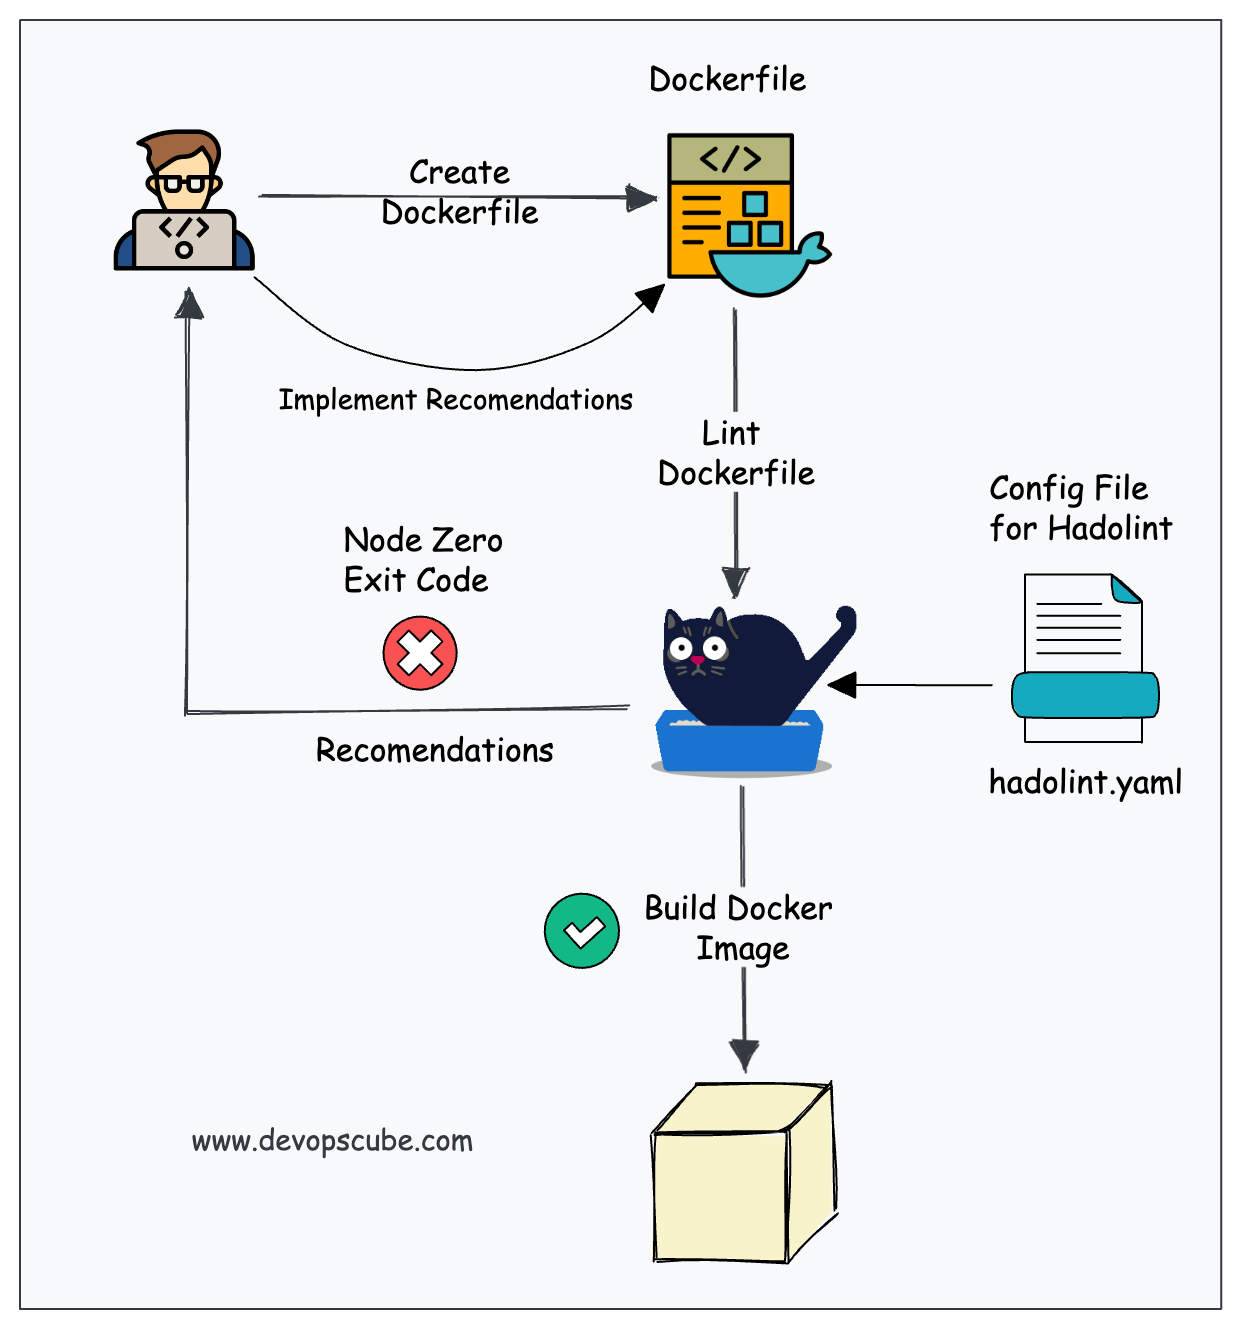
\includegraphics[width=0.58\textwidth]{Figures/hadolint-workflow.png}
  \caption{Workflow for Hadolint \cite{wilson_2023}} % Use braces {} for the caption text
  \label{fig:2.5} % Ensure unique label
\end{figure} 

Despite these advantages, Hadolint has limitations. As illustrated in Figure \ref{fig:2.5}, the workflow highlights how Hadolint integrates into the Dockerfile linting process, providing checks for syntax and best practices. However, it lacks vulnerability scanning capabilities and focuses solely on Dockerfile syntax and best practices. The tool flags issues but does not provide in-depth guidance or prioritize fixes based on their impact on performance or security, leaving developers to rely on their expertise. Moreover, Hadolint offers static feedback, providing insights only when invoked rather than real-time guidance during the development process. These limitations, while significant, provide a foundation for exploring the additional capabilities offered by other tools.

With an emphasis on both operating system packages and application dependencies, Snyk is an expert at locating and fixing vulnerabilities in container images. It can identify problems with a variety of components thanks to its extensive vulnerability database, which is updated frequently. Snyk smoothly connects with many container registries, including DockerHub and AWS ECR, and offers workable solutions, such as patching and version upgrades. Its continuous monitoring feature, which notifies users of fresh vulnerabilities in previously scanned photos even when no modifications have been made to the image itself, is a notable feature. Snyk has also improved its coverage of container security by adding the ability to check Dockerfiles for vulnerabilities.\cite{snyk_2024}
\begin{figure}[ht]
  \centering
   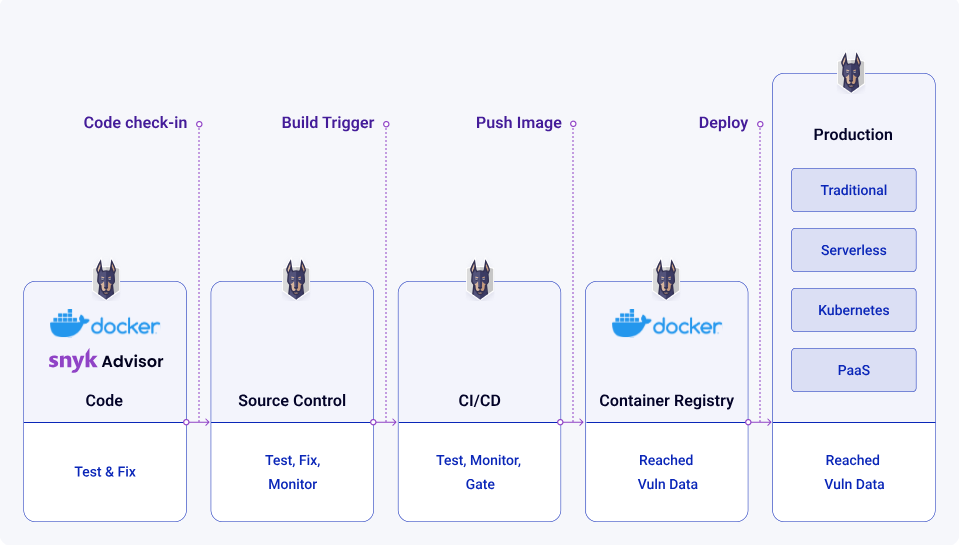
\includegraphics[width=0.9\textwidth]{Figures/snyk.png}
  \caption{Workflow for Snyk \cite{snyk2023}} % Use braces {} for the caption text
  \label{fig:2.6} % Ensure unique label
\end{figure} 

As illustrated in Figure \ref{fig:2.6}, Snyk integrates into the development workflow to provide vulnerability scanning and remediation recommendations.

But the main goal of Synk's Dockerfile scanning is to find vulnerabilities associated with base images and dependencies. It is unable to enforce recommended practices that affect performance and maintainability or identify "Docker smells". For example, Snyk doesn't examine the structure of Dockerfiles or suggest changes to reduce image size or boost build speed. Snyk does not offer comprehensive insights on compliance with best practices for Dockerfile setups, in contrast to tools such as Hadolint.\cite{snyk2023}

Synk's static rule set for Dockerfile scanning is another drawback. Although it is good at identifying known vulnerabilities, unlike the proposed Docker Linter, it does not update its rules on a regular basis to reflect changing best practices for Dockerfile optimisation. Furthermore, developers must rely on post-commit scans because Snyk does not provide real-time feedback during Dockerfile construction. This might complicate iterative development and postpone issue resolution. These shortcomings draw attention to the necessity of tools such as the Docker Linter, which place an emphasis on real-time feedback, ongoing rule modifications, and comprehensive Dockerfile analysis for efficiency and security.

The proposed Docker Linter aims to bridge gaps in existing tools by offering a specialized solution solely for Dockerfile linting and optimization. Unlike Hadolint, which provides a general static analysis of Dockerfiles, and Snyk, which primarily focuses on container image vulnerabilities, this tool focuses entirely on improving the structure and practices within Dockerfiles. By honing in on Dockerfile quality, the Docker Linter addresses inefficiencies such as unpinned base images, excessive layers, deprecated instructions, and other "Docker smells" that directly impact the performance and maintainability of resulting container images.

A unique feature of the Docker Linter is its ability to prioritise issues based on their severity and their predicted impact on performance, maintainability, and security outcomes of the built images. This prioritisation helps developers focus on critical improvements during the Dockerfile authoring process. Additionally, the linter distinguishes itself by continuously updating its rules through web scraping, ensuring adherence to the latest Docker best practices and industry standards.

Although tools such as Hadolint and Snyk are capable of delivering real-time feedback during the course of development or throughout CI/CD procedures, they depend on static or predetermined rule sets that can become outdated as time progresses. The Docker Linter, however, employs a dynamic rule update mechanism that guarantees developers have access to the most recent guidelines. This strategy, when integrated with real-time feedback provided within Integrated Development Environments (IDEs), enables developers to proactively refine Dockerfiles by addressing issues as they come up, thereby ensuring the production of high-quality container images that adhere to continuously advancing standards.

\begin{table}[ht]
    \centering
        \begin{tabular}{|p{3.5cm}|p{3.5cm}|p{3.5cm}|p{3.5cm}|}
            \hline
            \textbf{Feature} & \textbf{Hadolint} & \textbf{Snyk} & \textbf{Proposed Docker Linter} \\ \hline
            \textbf{Primary Focus} & Dockerfile linting for best practices & Vulnerability detection in container images and dependencies & Combined Dockerfile smell detection and vulnerability analysis \\ \hline
            \textbf{Smell Detection} & Yes (rule-based) & No & Yes, with dynamic rule updating \\ \hline
            \textbf{Vulnerability Scanning} & No & Yes & No \\ \hline
            \textbf{Automated Refactoring} & No & Yes & No \\ \hline
            \textbf{Continuos Rule updating} & No & No & Yes \\ \hline
            \textbf{IDE Integration} & Yes & Yes & Yes (real-time feedback) \\ \hline
            \textbf{CI/CD Integration} & Yes & Yes & Yes \\ \hline
            \textbf{Security Focus} & Limited to Dockerfile practices & Comprehensive (image and dependencies) &Limited to Dockerfile practices \\ \hline
            \textbf{Performance Optimization} & Limited to reducing image size & No & Yes (layer optimization, caching improvements) \\ \hline
            \end{tabular}
        \caption{Comparison of Hadolint, Snyk, and Proposed Docker Linter}
        \label{tab:tool_comparison}
\end{table}

The Docker Linter offers detailed explanations for each flagged issue, making it easier for developers to understand and address problems. Unlike Snyk, which focuses on image vulnerabilities, the Docker Linter emphasizes performance optimization and Dockerfile-specific analysis, ensuring that images are not only secure but also efficient and maintainable. Additionally, the tool incorporates Docker smell detection, providing developers with insights into inefficiencies at the Dockerfile level and helping them make informed decisions about prioritizing fixes.

The comprehensive capabilities of the Docker Linter are summarized in Table \ref{tab:tool_comparison}, which highlights the key features and limitations of Hadolint, Snyk, and the proposed tool. This comparison underscores the Docker Linter’s potential to serve as a comprehensive solution for improving Dockerfile quality and container security, addressing the limitations of existing tools while enhancing their strengths.

\subsubsection{Addressing Security in Docker Artifacts}
Docker containers are widely used for their efficiency and scalability, but they come with inherent security risks. The research by Rosa et al. highlights critical security issues stemming from Docker smells and proposes best practices to mitigate these risks\cite{DockerArtifacts}.This section explores the security vulnerabilities associated with Docker artifacts, examines proposed solutions in the literature, and outlines how the proposed Docker Linter can enhance security in Dockerfiles.

"Docker smells", such as running containers with root privileges, unpinned dependencies, and unnecessarily exposed ports, present significant security threats. These practices increase the attack surface, leaving containers vulnerable to exploits.\cite{Dockeranalysis}

\begin{enumerate}
    \item \textbf{Running Containers as Root:}By default,Docker containers run with root privileges, providing attackers with potential administrative access.This setup increases the likelihood of privilege escalation attacks. Privilege escalation attacks refers to a network attack aiming to gain unauthorised higher-level access within security systems.It can start with attackers exploiting vulnerabilities like running containers as root. The attackers then evaluate their access rights to gain control over sensitive information. \cite{Dockeranalysis}

    \item \textbf{Unpinned Dependencies:}The failure to pin versions of base images or software dependencies is a significant security risk in containerized environments. When a Dockerfile does not specify exact versions of the base image or installed packages, it implicitly pulls the latest available version at build time. This introduces several challenges:
    \begin{itemize}
        \item \textbf{Inconsistency in Builds:}Without version pinning, each build can result in a different image composition depending on the latest version available. This lack of reproducibility complicates debugging and quality assurance, as not all builds will be identical across different environments.For example, if a vulnerability is introduced in an newer version of a base image, containers built at different times could have different levels of security. 
        \item \textbf{Increased Vulnerability Exposure:}Unpinned dependencies make containers vulnerable to newly introduced vulnerabilities. For instance, a developer might unknowingly build a container using a base image or dependency version containing a critical security flaw, exposing the container and its host environment to potential exploits. The recent surge in supply chain attacks has further underscored the dangers of relying on unverified or automatically updated components.
        \item \textbf{Uncontrolled Updates:}Unpinned dependencies allow updates to occur automatically during builds, which might include breaking changes or introduce new bugs. These unintended changes can disrupt the application’s functionality or create unexpected security risks. Developers may find themselves scrambling to resolve issues caused by automatic updates during critical deployment phases.
        \item \textbf{Impact on Dependency Trees:}A single unpinned dependency can propagate through the dependency tree, introducing multiple layers of vulnerabilities. For example, if a base image pulls unpinned system libraries or utilities, vulnerabilities in those libraries might remain hidden until they are exploited.
    \end{itemize}
    \item \textbf{Exposed Ports and Services:}Exposing unnecessary ports in Dockerfiles can significantly increase the risk of network-based attacks. Docker containers often include services that communicate with the outside world through specific ports. If these ports are left exposed without proper justification or security measures, they become potential entry points for attackers. Here’s how this vulnerability manifests\cite{Dockeranalysis}:
    \begin{itemize}
        \item \textbf{Increased Attack Surface:} Every open port in a container represents a potential area to be exploited.Exposed ports can provide attackers with direct access to internal services or applications running within the container.This access is dangerous if the exposed service has known vulnerabilities or is misconfigured.For example, exposing admin ports without proper authentication can enable attackers to gain unauthorised control over the container.
        \item \textbf{Man in the middle attacks:}When a container communicates with external services over exposed ports, attackers can interpret this communication, particularly if it occurs over unencrypted channels. In a Man in the middle attack, the attacker positions themselves between the container and its intended recipient, capturing sensitive data such as login credentials, API keys, or private user information.Containers that expose ports for services like databases or APIs are especially vulnerable if these services lack proper encryption or authentication.

        \item \textbf{Port Scanning Exploits:}Attackers frequently use automated tools to scan for open ports on exposed containers. Once identified, these ports can be targeted for specific vulnerabilities associated with the services they host.For example, a port scan might reveal that a container is running an outdated version of a web server with known security flaws, enabling attackers to exploit these weaknesses.

    \end{itemize}
\end{enumerate}

To reduce the security risks associated with unpinned dependencies, industry best practices emphasise the importance of explicit version pinning, automated scanning, and regular updates. Developers should specify exact versions of base images and dependencies in Dockerfiles (e.g., FROM ubuntu:20.04 instead of FROM ubuntu:latest) to ensure consistent builds and minimize exposure to vulnerabilities. Automated tools like Snyk and Hadolint can help identify outdated or vulnerable dependencies, enabling timely remediation. Additionally, organisations should periodically review and update pinned dependencies to incorporate security patches and performance improvements, testing these updates in staging environments before production deployment. Together, these practices enhance container security and maintain application stability

\subsubsection{Enhancing Developer Productivity and CI/CD Pipelines}
Maintaining Dockerfiles efficiently is a significant challenge for developers, particularly in complex micro-services environments where hundreds of services must interact seamlessly. Each Dockerfile serves as a critical component for defining containerized applications, and any deviation from best practices can lead to recurring issues, including slower build times, increased resource consumption, and higher operational costs. A key hurdle is the time-intensive manual reviews that developers must perform to ensure Dockerfiles meet industry standards. These reviews often depend on individual expertise, leading to inconsistencies across projects. As a result, organizations face varied levels of compliance, increasing the likelihood of performance bottlenecks, security vulnerabilities, and unplanned downtime due to misconfigured containers

Furthermore, developers often lack visibility into the long-term consequences of "Docker smells", such as unoptimized layering, unpinned dependencies, or excessive permissions. These inefficiencies might not cause immediate failures but tend to accumulate over time, degrading system performance, bloating images, and increasing security risks. For organizations operating at scale, even minor inefficiencies in Dockerfile configurations can amplify into substantial performance penalties, particularly in cloud environments where resource optimization directly impacts costs.

The arrival of automated linting tools has revolutionized this space by offering developers a more streamlined way to enforce best practices. Tools like Hadolint analyse Dockerfiles against a predefined set of rules, automatically flagging violations such as outdated base images, excessive layers, and insecure configurations. However, these tools primarily operate in static, post-development environments, providing feedback after Dockerfiles have been written and pushed to repositories. This delayed feedback loop often leads to iterative cycles of error detection, debugging, and rework, prolonging development timelines.

The Docker Linter makes things easier for developers by giving real-time feedback right inside their coding environment, like their IDE. This means they can fix problems in their Dockerfiles as they write them. For example, if a developer uses a RUN command but forgets to clean up temporary files, the linter will immediately point it out and suggest a fix, like adding \verb|rm -rf /var/lib/apt/lists/*|. This helps keep Dockerfiles clean and efficient from the start, without waiting for later checks.

In the context of Continuous Integration and Continuous Deployment (CI/CD) pipelines, the Docker Linter plays an essential role in maintaining a high standard of quality across all deployments. CI/CD pipelines benefit greatly from automated linting as it enforces consistent best practices and prevents common errors from popping up into production. The Docker Linter integrates seamlessly into popular CI/CD tools like Jenkins, Git Lab CI, and GitHub Actions, automating the process of checking Dockerfiles for compliance at every stage of the software development lifecycle. This ensures that even in fast-paced environments where multiple teams are working on concurrent deployments, every build meets organizational quality and security standards.\cite{2022continuous}

The linter’s capabilities focus on providing developers with clear identification,prioritization of issues and providing continuous rule updates, such as redundant layers or unpinned dependencies. By highlighting the most up-to-date "smells" and ranking them based on their severity, the tool enables developers to address the most critical problems efficiently. This approach ensures that Dockerfiles are consistently optimized while maintaining a streamlined development workflow without adding unnecessary overhead..

Another significant advantage lies in the tool’s ability to streamline collaboration across distributed teams. By ensuring that all developers follow the same set of rules and receive consistent feedback, the Docker Linter reduces variability in Dockerfile quality across different projects and teams. This uniformity simplifies the debugging and troubleshooting process, as developers can rely on a common structure and set of practices for Dockerfile configurations.

Ultimately, the Docker Linter enhances developer productivity by minimizing the time and effort spent on manual reviews, reducing error rates, and ensuring that containerized applications are efficient, secure, and maintainable. It empowers organizations to achieve faster and more reliable deployments, improving the agility and scalability of their CI/CD pipelines, and reinforcing their commitment to delivering high-quality software at scale.

\subsubsection{Implications for Organizations}

The paper "Assessing and Improving the Quality of Docker Artifacts" emphasizes the critical importance of maintaining high-quality Docker artifacts for modern software development. As containerized applications continue to grow in adoption, enhancing Dockerfile and Docker image quality has become a strategic priority for organizations. Improving quality directly impacts security, cost efficiency, and operational performance, making it a cornerstone of effective container management strategies. This section explores the organizational benefits based on the findings of Rosa et al.\cite{DockerArtifacts}.

One of the most significant organizational benefits of improving Docker artifacts is enhanced security. Adhering to industry-standard best practices in Dockerfile creation helps to mitigate vulnerabilities that could arise from poor configurations. Common "Docker smells," such as unpinned dependencies or containers running with excessive privileges (e.g., root access), pose substantial risks to application security. This project addresses these issues by enabling automated detection of such smells through a linter that continuously updates its rule set via a web scraper. This ensures that the tool reflects the latest industry best practices, equipping organizations to proactively safeguard their applications against emerging threats.

Another key benefit is cost efficiency, especially in cloud environments where resource optimization directly translates to reduced expenses. Optimized Dockerfiles lead to smaller image sizes, which lower storage requirements, accelerate deployment times, and reduce network transfer costs. Rosa et al. highlight how these improvements enable organizations to achieve better resource utilization and cost savings, particularly in large-scale deployments. By focusing on eliminating unnecessary layers, enforcing multi-stage builds, and reducing redundant dependencies, the Docker Linter contributes to creating lean, high-performance images suitable for modern cloud-native strategies.

Improved Dockerfile quality also enhances development workflows by reducing the overhead associated with manual code reviews and debugging. The integration of the Docker Linter into CI/CD pipelines ensures that Docker artifacts consistently meet high-quality standards without requiring extensive manual intervention. This allows developers to concentrate on feature development rather than addressing recurring infrastructure issues. The tool's real-time feedback mechanism within IDEs further supports a streamlined development process, enabling developers to identify and fix potential issues as they write Dockerfiles, ensuring compliance with best practices from the outset.

This project's unique use of a web scraper for continuous rule updates is particularly valuable in maintaining organizational alignment with the industry's evolving best practices. Unlike other tools that rely on static rules or require manual updates, the Docker Linter ensures that developers are always working with the most up-to-date standards. This proactive approach not only enhances the relevance of the tool but also reduces the risk of technical debt associated with outdated practices.

Organizations adopting containerization strategies, particularly in hybrid and multi-cloud environments, face the challenge of ensuring consistent Dockerfile quality across diverse platforms. The Docker Linter addresses this challenge by enabling developers to produce optimized and standardized Dockerfiles, regardless of the underlying infrastructure. This ensures smoother workload migrations between cloud providers while maintaining high performance and security standards.

Additionally, the Docker Linter supports operational efficiency by helping organizations achieve faster deployment cycles and more reliable applications. By eliminating inefficiencies and enforcing best practices, the tool reduces downtime and improves application stability, allowing organizations to deliver high-quality software at scale.

The insights from Rosa et al. underscore the importance of high-quality Docker artifacts in modern software development. By adopting tools like the Docker Linter, organizations can not only enhance their container management practices but also achieve broader business goals, including cost reduction, improved security, and increased developer productivity. This project aligns closely with these objectives, providing organizations with a robust solution for maintaining consistent, high-quality Docker artifacts in a rapidly evolving industry landscape.